\chapter{Introduction}
\label{sec:introduction}
\newpage

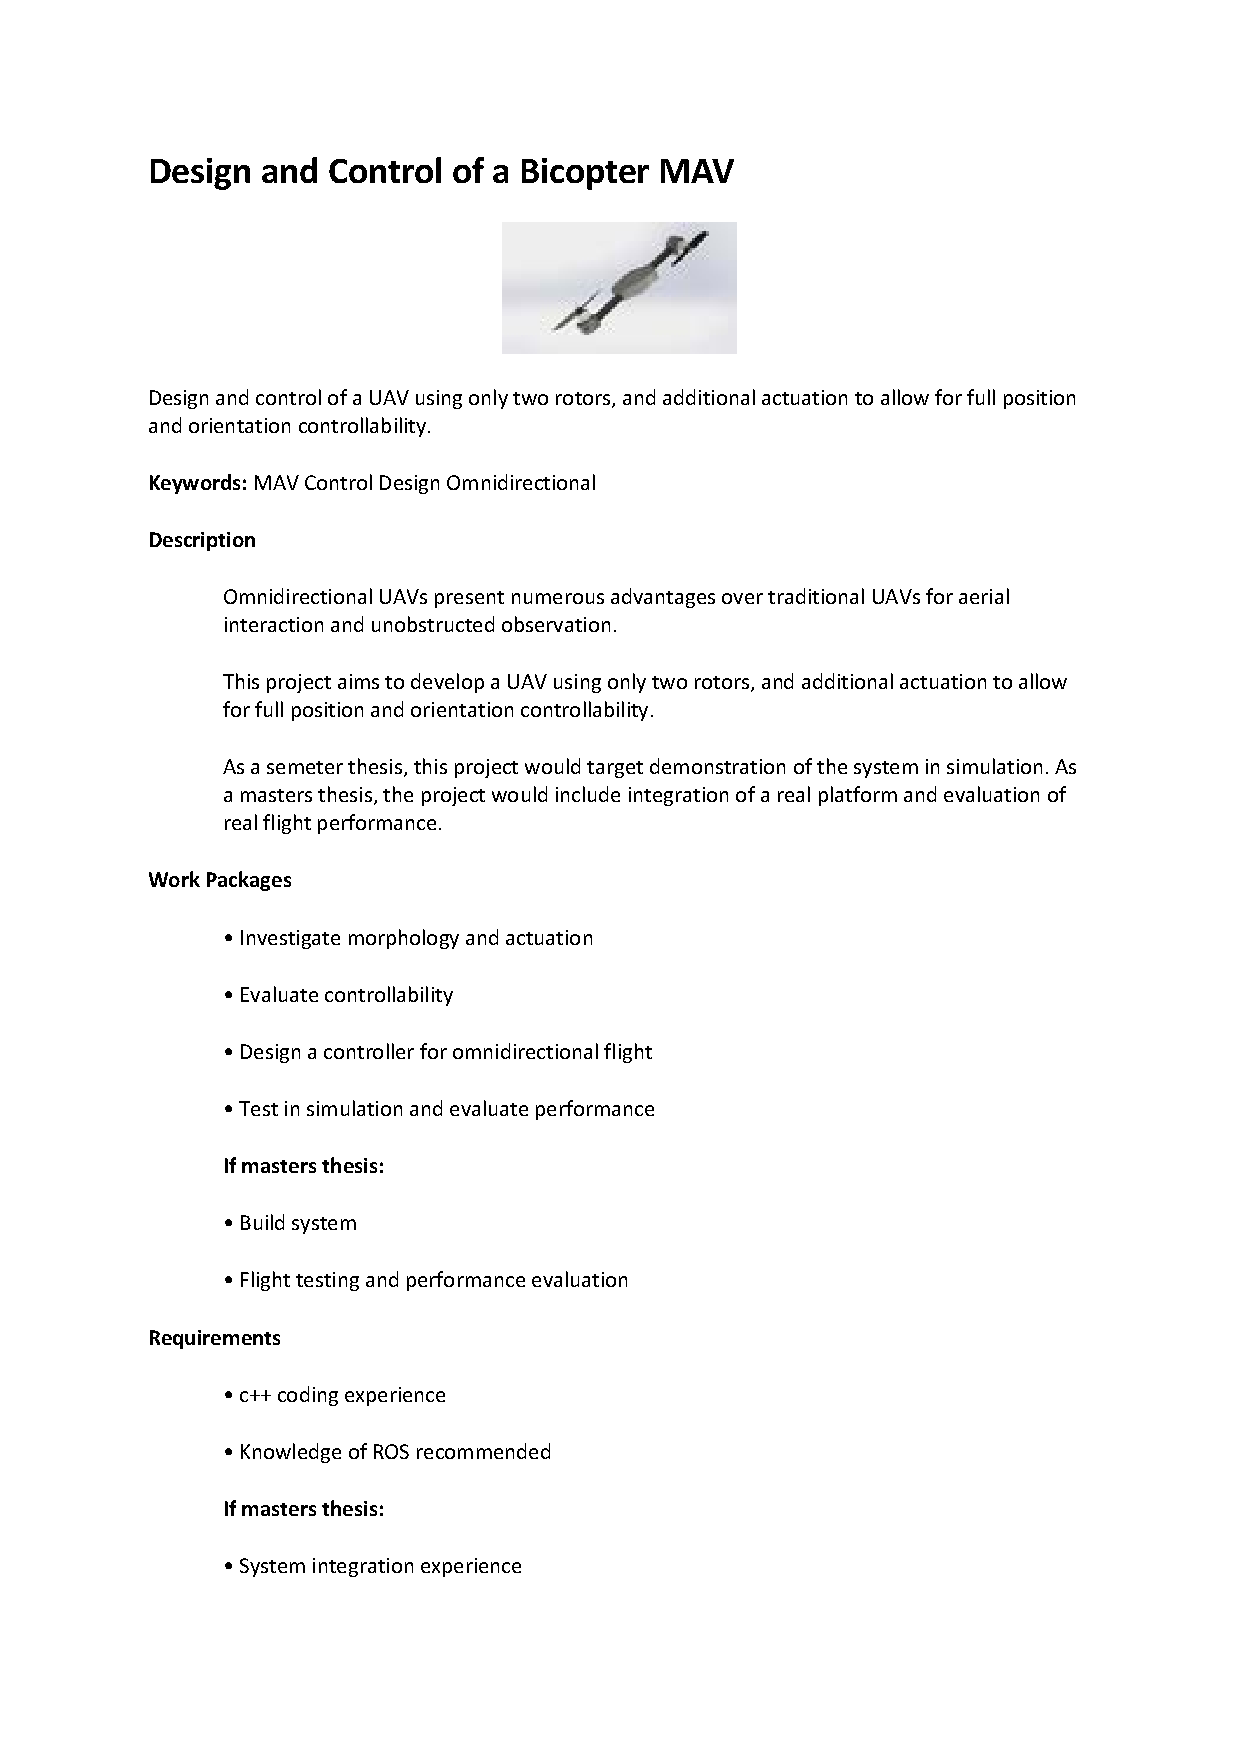
\includepdf[scale=0.7, pagecommand={\section{Description of the project by ASL} \thispagestyle{empty}}, fitpaper=true]{images/introduction/advertisementBicopter.pdf}

\section{Goals}
% The purpose of this project was to create a bicopter that could flight in each direction and changed the yaw angle.
???

\section{Workflow}
Worked every weeks on it.
Present my progress and advancement each week to my supervisors
\section{Timeline}
At the start of the project, the expected plan showed in the figure \ref{pics:expectedGantt} was ambitious. Therefore it was difficult to respect it along the semester because it also was some courses to attend and we added to build a prototype during the first part of the semester.
\begin{figure}[h!]
   \centering
   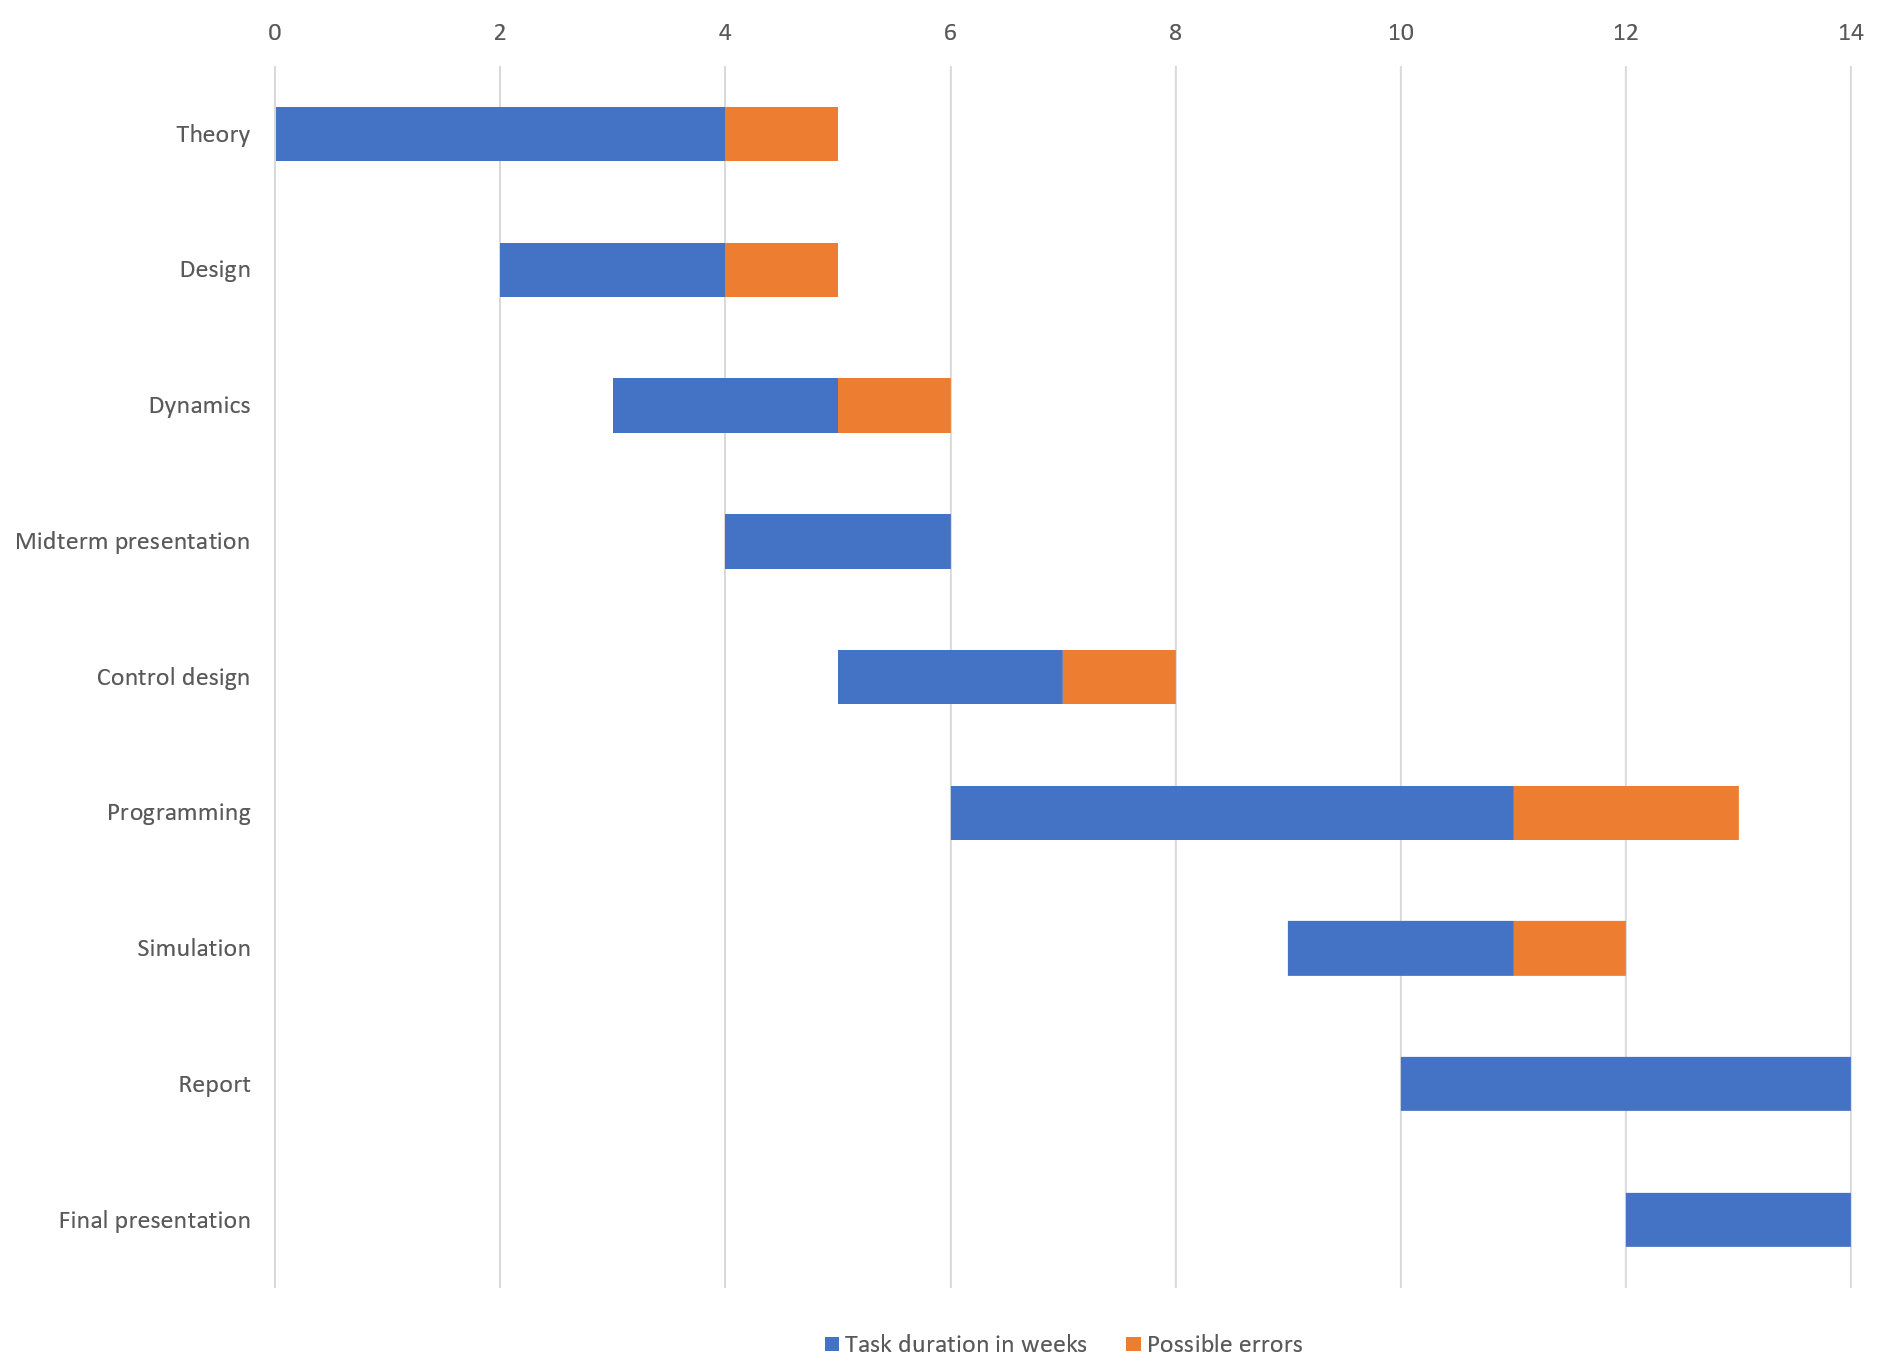
\includegraphics[width=0.9\textwidth]{images/introduction/expectedGantt}
   \caption{Expected plan for the semester project}
   \label{pics:expectedGantt}
\end{figure}

So, the real planning would become ...

\begin{figure}[h!]
   \centering
   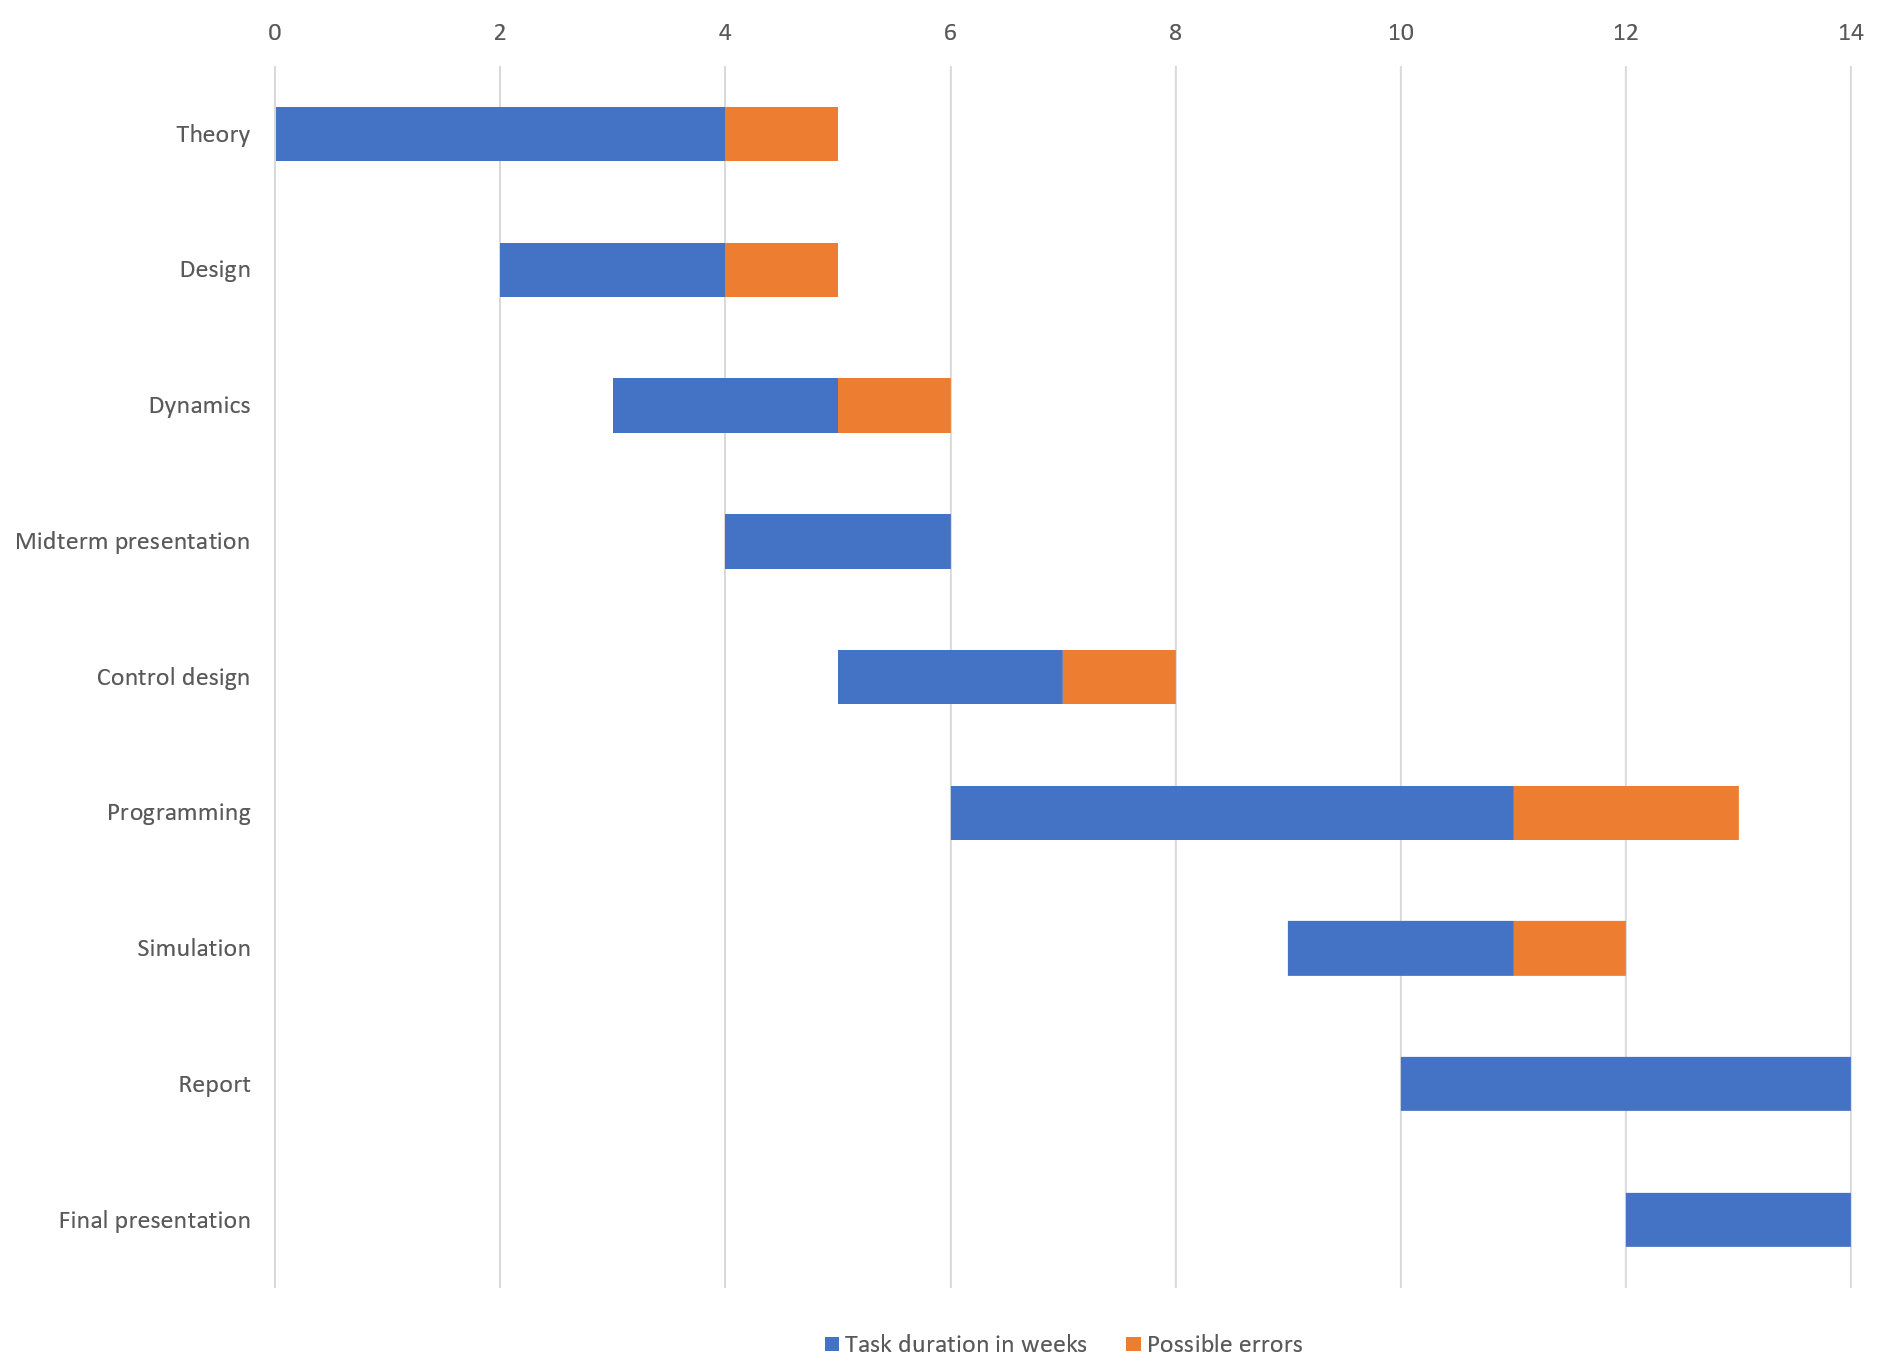
\includegraphics[width=0.9\textwidth]{images/introduction/expectedGantt}
   \caption{Real plan for the semester project}
   \label{pics:realGantt}
\end{figure}

\clearpage